%Part of/Parte di https://github.com/f-dinucci/appuntiMeccanicaFluidi/
%License/Licenza Creative Commons Attribution-ShareAlike 4.0 International (CC BY-SA 4.0) - attribution/attribuzione Francesco Di Nucci
%See also/Vedere anche https://creativecommons.org/licenses/by-sa/4.0/ and/e https://creativecommons.org/licenses/by-sa/4.0/legalcode
%
\section{Ingressi e uscite concentrati}

%SUBSECTION
\subsection{Pareti impermeabili}
Per definizione una parete impermeabile non può essere attraversata dal fluido, quindi non vi è flusso di massa. 
Da un punto di vista matematico:
%
	\begin{equation*}
		\uline{v}_r \vdot \uline{n} = 0
	\end{equation*}
%
Ricordare che come caso particolare se la parete non si muove $\uline{v}_r = \uline{v}$

%SUBSECTION
\subsection{Approssimazione di ingressi e uscite concentrati}
Si vedrà ora cosa accade alle equazioni di bilancio nel caso in cui si faccia l'ipotesi di avere un contenitore racchiuso da una parete impermeabile e con ingressi ed uscite relativamente piccoli rispetto a questa.
%
	\begin{figure}[ht]
		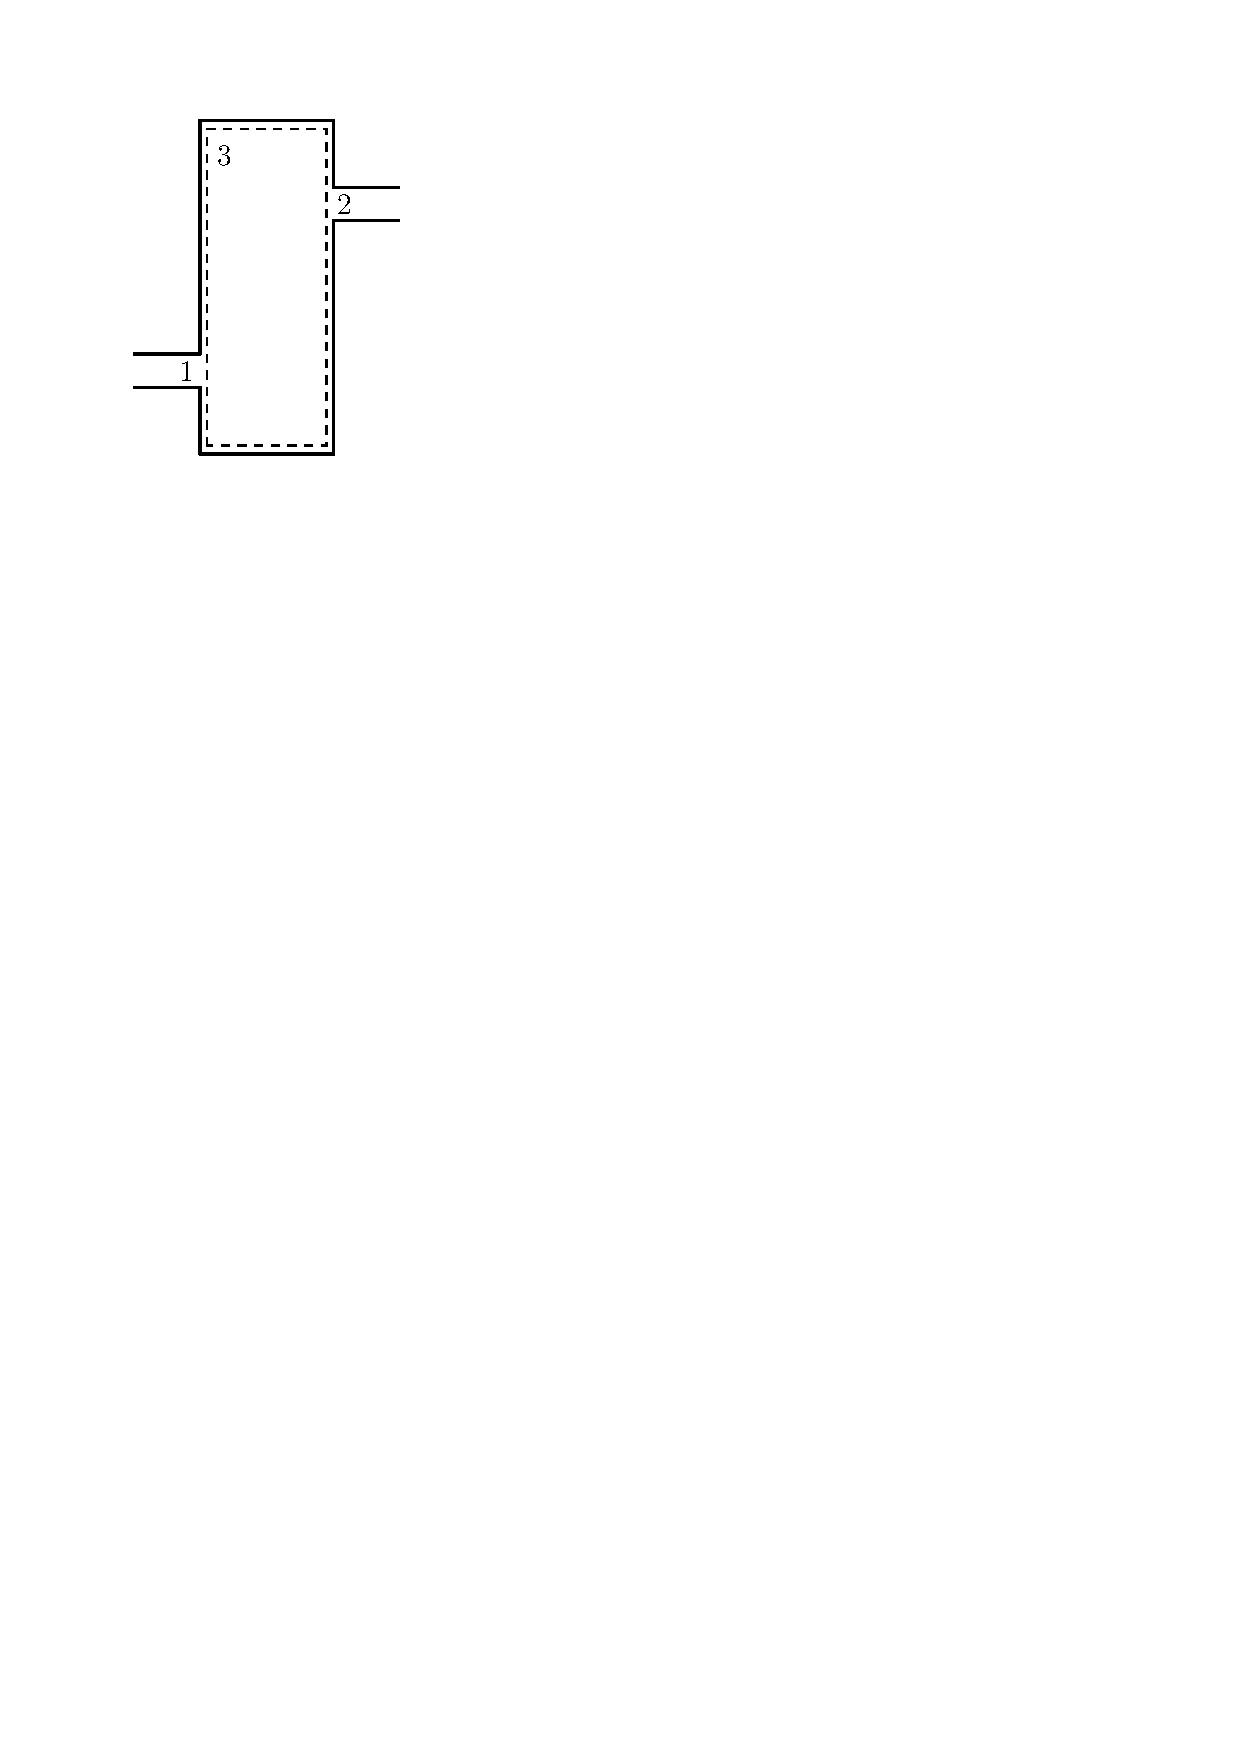
\includegraphics[scale=0.9]{./3.2 Ingressi e uscite concentrati/3.2-1}
		\centering
		\caption{Contenitore con ingressi e uscite concentrati}
	\end{figure}
%
Occorre vedere caso per caso dove questa approssimazione sia valida, se ne discuterà successivamente. 
Per ora si inizi suddividendo l'integrale sul contorno chiuso nelle parti che lo compongono, sfruttando la proprietà di additività degli integrali:
%
	\begin{equation*}
		\oint (\ldots) \dd{S} = \int_1 (\ldots) \dd{S} + \int_2 (\ldots) \dd{S} \int_3 (\ldots) \dd{S}
	\end{equation*}
%

\subsubsection{Massa}
Scomponendo nei vari integrali e ricordando la definizione di parete impermeabile:
%
	\begin{equation*}
		\dv{t} \int \rho \dd{V} + \int_1 \rho \uline{v}_r \vdot \uline{n} \dd{S} + \int_2 \rho \uline{v}_r \vdot \uline{n} \dd{S} + \cancel{\int_3 \rho \uline{v}_r \vdot \uline{n} \dd{S}} = 0
	\end{equation*}
%
Riscrivendo poi per comodità $\dv{M}{t} = \dv{t} \int \rho \dd{V}$ e sostituendo alla velocità in ingressi/uscite il suo valore medio, dato che si suppone che in questi la velocità vari poco:
%
	\begin{equation*}
		\dv{M}{t} + \rho_1 \uline{v}_{r1} \vdot \uline{n}_1 S_1 + \rho_2 \uline{v}_{r2} \vdot \uline{n}_2 S_2 = 0
	\end{equation*}
%
\subsubsection{Quantità di moto}
Analogamente si procede per la quantità di moto:
%
	\begin{equation*}
		\begin{aligned}
			\dv{t} \int \rho \uline{v} \dd{V} + \int_1 (p \uline{n} + \rho \uline{v} \uline{v}_r \vdot \uline{n}) \dd{S} + \int_2 (p \uline{n} + \rho \uline{v} \uline{v}_r \vdot \uline{n}) \dd{S} +  \\
			+ \int_3 (p \uline{n} + \rho \uline{v} \uline{v}_r \vdot \uline{n}) \dd{S} = \int \rho \uline{g} \dd{V} 
		\end{aligned}
	\end{equation*}
%
In ingressi e uscite si può supporre che pressione e velocità non varino molto e possano quindi essere sostituite con il loro valore medio. 
Dato che la parete è impermeabile $\rho \uline{v} \uline{v}_r \vdot \uline{n}$.
Riscrivendo per comodità $\int \rho \uline{g} \dd{V} = \uline{F}_g$ si ha:
%
	\begin{equation*}
		\dv{t} \int \rho \uline{v} \dd{V} + ( p_1 \uline{n}_1 + \rho \uline{v}_1 \uline{v}_{r1} \vdot \uline{n}_1 ) S_1 + ( p_2 \uline{n}_2 + \rho \uline{v}_2 \uline{v}_{r2} \vdot \uline{n}_2 ) S_2 + \int_3 p \uline{n} \dd{S} = \uline{F}_g
	\end{equation*}
%
In questa $\int_3 p \uline{n} \dd{S} = \uline{F}_C$ è la forza esercitata sulle pareti del contenitore, come integrale non è trascurabile né approssimabile, dato che riguarda una superficie estesa, ma non è un problema dato che è quasi sempre l'incognita da calcolare.
Se si è in un caso stazionario, in cui per definizione la velocità non varia con il tempo ma solamente con lo spazio, $\dv{t} \int \rho \uline{v} \dd{V} = 0$. Questo non va confuso con il caso statico, in cui la velocità è nulla, dato che il fluido è fermo.

\subsection*{Bibliografia 3.3}
\cite[Cap.\ 5.2]{CengelCimbala}\\
\cite[Cap.\ 4.3, 4.4]{PnueliGutfinger}